\chapter{Architektura}
\label{cha:architektura}
Na podstawie analizy możliwych rozwiązań sprzętowych w~rozdziale \ref{cha:specyfikacja} oraz przedstawionych poniżej założeń architektury platformy dokonano wyboru urządzeń, które będą stanowiły część sprzętową tworzonego interfejsu.

\section{Założenia architektury sprzętowej}
Aby wybrać odpowiedni dla przygotowywanego prototypu interfejsu zestaw urządzeń, określone zostały założenia i~wymagania, jakie urządzenia powinny spełniać:
\begin{enumerate}
\item Urządzenie powinno być lekkie, aby używanie go przez gracza nie powodowało dyskomfortu, który może wpłynąć negatywnie na jakość odbieranych danych.
\item Dokładność sensorów dostępnych w~urządzeniu powinna być jak największa, aby mieć pewność odczytywanych zachowań użytkownika.
\item Urządzenie powinno być łatwe w~obsłudze, zarówno w~kwestii jego zamontowania, jak i~uruchomienia odczytów. Powinno być także jak najmniej inwazyjne podczas pomiaru, aby zminimalizować dyskomfort użytkownika.
\item Dla wybranego urządzenia powinno być dostępne oprogramowanie umożliwiające odczyt pomiarów w~wybranym środowisku do tworzenia gier. Najlepiej, gdyby rozwiązanie było dostępne w~postaci biblioteki oferowanej przez twórcę sprzętu, lub rozszerzenia silnika, które umożliwi odczyt danych z~urządzenia.
\item Urządzenie powinno mieć możliwość połączenia bezprzewodowego, najlepiej przy pomocy technologii Bluetooth, lub innego protokołu umożliwiającego bezprzewodowy odczyt pomiarów z~urządzenia.
\item Przynajmniej jedno z~urządzeń powinno umożliwiać odczyt pracy serca, w~postaci pomiaru pulsu lub elektrokardiogramu. Pomiar pracy serca jest jedną z~podstawowych metod umożliwiających określenie zmiany w~stanie emocjonalnym użytkownika.
\item Przynajmniej jedno z~urządzeń powinno umożliwiać pomiar ruchów mięśni. Odczytane sygnały mogą być wykorzystane do wpływania na rozgrywkę w~zależności od aktywności mięśniowej użytkownika w~danej partii ciała.
\end{enumerate}


\section{Garmin HRM-Run}
Garmin HRM-Run jest jednym z~wielu dostępnych czujników tętna produkowanych przez firmę Garmin. Urządzenie zbudowane jest z~modułu zawierającego całą elektronikę odpowiedzialną za interpretację oraz wysyłanie odczytywanych danych. Moduł zasilany jest baterią CR2032 i~zamontowany jest na elastycznej opasce, umożliwiającej zamontowanie opaski na klatce piersiowej. Sama opaska zawiera dwie elektrody, które odpowiadają za odczyt sygnałów fizjologicznych, które następnie są przekazywane w~formie informacji na temat pracy serca. 

Urządzenie, poza podstawowym pomiarem liczby uderzeń na minutę, pozwala na odczyt dodatkowych informacji na temat zmienności rytmu zatokowego w~postaci odstępów czasowych pomiędzy kolejnymi tzw. załamkami R, czyli szczytami kompleksów QRS. Na podstawie tej informacji można określić stan zdrowotny użytkownika lub zmiany jego stanu emocjonalnego. Dla przykładu nagłe spadki w~zmienności rytmu zatokowego mogą sygnalizować możliwość odczuwania stresu przez użytkownika. HRM-Run umożliwia także odczyt pomiarów dynamiki biegu takich jak liczba kroków na minutę, czas kontaktu z~podłożem czy długość kroku. Ze względu na charakter pracy, która skupia się głównie na tematyce gier komputerowych, pomiary te nie były brane pod uwagę. 

Urządzenie HRM-Run zostało wybrane, ponieważ stanowi pewien kompromis pomiędzy dokładnością odczytów a~rozmiarami i~wygodą użytkowania. W~porównaniu do inteligentnych opasek, które charakteryzują się najwyższą wygodą użytkowania spośród omówionych w~rozdziale \ref{cha:specyfikacja} urządzeń umożliwiających pomiar tętna, Garmin HRM-Run pozwala na o~wiele dokładniejsze odczyty, nie powodując jednocześnie dyskomfortu podczas użytkowania. Jest to możliwe dzięki wykorzystaniu elastycznej opaski ze wbudowanymi suchymi elektrodami, które w~przeciwieństwie do fotopletyzmografu odpowiadającego za optyczny odczyt tętna w~inteligentnych opaskach, odbierają sygnały elektryczne bezpośrednio z~ciała użytkownika, które są następnie interpretowane do danych w~postaci wykrycia kolejnych uderzeń serca. Opaski charakteryzują się także dużymi opóźnieniami w~stosunku do aktualnego tętna użytkownika, co w~przypadku rozpoznawania emocji w~sposób ciągły całkowicie eliminuje je jako akceptowalne urządzenia. Jednocześnie, elastyczna opaska, do której przymocowany jest moduł, w~bardzo prosty sposób jest zakładana przez użytkownika na klatce piersiowej, Takie umiejscowienie i~brak kabli łączących elektrody z~głównym modułem sprawia, że użytkownik nie czuje dyskomfortu podczas noszenia urządzenia. W~podobny sposób Garmin HRM-Run można porównać z~omawianym wcześniej BITalino (r)evolution kit. W~tym przypadku można zauważyć sytuację odwrotną, niż przy porównaniu z~inteligentnymi opaskami. BITalino oferuje bardzo dokładny odczyt pracy serca, nie tylko w~formie liczby uderzeń na minutę, ale pełnego elektrokardiogramu, który umożliwia o~wiele szerszą analizę pracy serca. Niestety, odczyt wymaga zamocowania przyklejanych elektrod, które połączone są przewodami z~sensorem, a~następnie z~samym BITalino. Taki sposób montażu może wpłynąć negatywnie na komfort podczas gry, co nie wystąpi w~przypadku urządzenia HRM-Run.

Innym aspektem, który zadecydował o~wyborze tego urządzenia, jest obsługa dwóch protokołów bezprzewodowego przesyłania danych. Poza standardowym połączeniem dzięki technologii Bluetooth HRM-Run wykorzystuje także protokół ANT+ rozwijany przez firmę Garmin. Jego główną zaletą jest brak ograniczeń co do ilości urządzeń, które mogą odczytywać dane z~czujnika. W~przeciwieństwie do technologii Bluetooth, która ogranicza połączenie do jednego, lub w~przypadku Bluetooth Smart do dwóch urządzeń, pomiar przy pomocy protokołu ANT+ umożliwia jednoczesne odczytywanie danych w~grze i~monitorowanie pracy serca przy pomocy innych urządzeń lub aplikacji korzystających z~tego protokołu. Twórcy ANT+ udostępniają szeroką dokumentację oraz biblioteki umożliwiające odczyt w~wielu językach programowania, od C++, C\#, aż po dedykowane implementacje dla systemu Android.

\begin{figure}
	\centering
	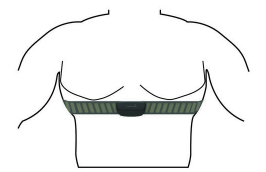
\includegraphics[width=0.5\linewidth]{images/garmin_hrm_placement.png}
	\caption{Miejsce montażu czujnika tętna Garmin HRM-Run, źródło:~\cite{garmin_manual}}
	\label{fig:garmin_placement}
\end{figure}

\section{BITalino (r)evolution kit}
BITalino (r)evolution Plugged Kit BT jest urządzeniem produkowanym przez firmę PLUX Wireless Biosignals przeznaczonym do tworzenia platform, w~których zawarte są elementy wymagające informacji na temat sygnałów fizjologicznych. Główny element narzędzia stanowi płytka zbudowana z~następujących elementów~\cite{bitalino_documentation}:
\begin{itemize}
	\item 10 złącz UC-E6, w~ramach których można wyróżnić: 6~wejść analogowych, 1~wejście cyfrowe, 1~wyjście cyfrowe, 1~złącze mogące pracować w~trybie wejścia lub wyjścia cyfrowego, oraz 1~złącze PWM, do którego może zostać podłączony przetwornik DAC lub dioda LED. Złącza są podzielone na 2~grupy w~oddzielnych segmentach.
	\item mikrokontroler z~mikroprocesorem oraz stykami umożliwiającymi połączenie każdego z~segmentów w~sposób inny niż standardowy.
	\item segment zasilający, zawierający włącznik, gniazdo ładownia w~formie złącza micro-USB oraz złącze JST, do którego podłączana jest bateria 3.7V zasilająca całą płytkę
	\item moduł Bluetooth odpowiadający za przesył danych z~płytki
\end{itemize}

W ramach przygotowywanego interfejsu, z~dostępnych sensorów opisanych w~rozdziale \ref{cha:specyfikacja} wybrany został jedynie moduł zawierający elektromiogram mierzący napięcie mięśni podskórnych. Głównym powodem takiego wyboru są dwie główne wady urządzenia z~perspektywy komfortu użytkowania. Są to przewody łączące płytkę z~sensorem, a~następnie z~elektrodami, oraz same elektrody. Choć z~perspektywy eksperymentów naukowych, użycie elektrod żelowych przyklejanych do skóry nie jest problemem, to w~przypadku środowiska gier komputerowych, standardowy użytkownik może odczuwać dyskomfort, lub w~ogóle zrezygnować z~używania urządzenia ze względu na jego inwazyjność. 

Głównym powodem wyboru BITalino oraz samego modułu EMG jest wykorzystanie sygnałów fizjologicznych do kontrolowania gry w~świadomy sposób. Odczyt zmian napięcia mięśni podskórnych może pozwolić na wykrycie, kiedy i~jak mocno są one używane, co może następnie zostać wykorzystane do zaimplementowania mechanik w~grze uruchamianych na podstawie konkretnych reakcji mięśniowych. Kolejnym powodem wykorzystania urządzenia jest możliwość sprawdzenia, w~jakim stopniu użytkownik tak naprawdę odczuwa dyskomfort podczas używania elektrod przyklejanych do skóry. Pozwoli to stwierdzić, czy urządzenia takie jak BITalino, które umożliwiają dokładny odczyt dzięki wykorzystaniu elementów bliższych rozwiązaniom medycznym, mogłyby przyjąć się jako stały element stanowiska do gier.

Ponieważ odczyty z~elektromiogramu mają posłużyć jako pewien element kontroli nad grą, jako miejsce, do którego podłączony będzie sensor, wybrano przedramię, ponieważ ruch mięśni znajdujących się w~tamtej części ciała może być precyzyjny. Dzięki temu użytkownik w prosty sposób, poprzez ruchy nadgarstka lub dłoni, może kontrolować napięcie mięśni w trakcie rozgrywki. Sposób montażu elektrod został przedstawiony na rysunku~\ref{fig:bitalino_placement}. Elektrody czerwona i czarna powinny znajdować się na wewnętrznej części przedramienia, równolegle do niego, stosunkowo blisko siebie. Elektroda referencyjna, w BITalino oznaczona kolorem białym, powinna znajdować się na wystającej kości łokciowej.
\begin{figure}
	\centering
	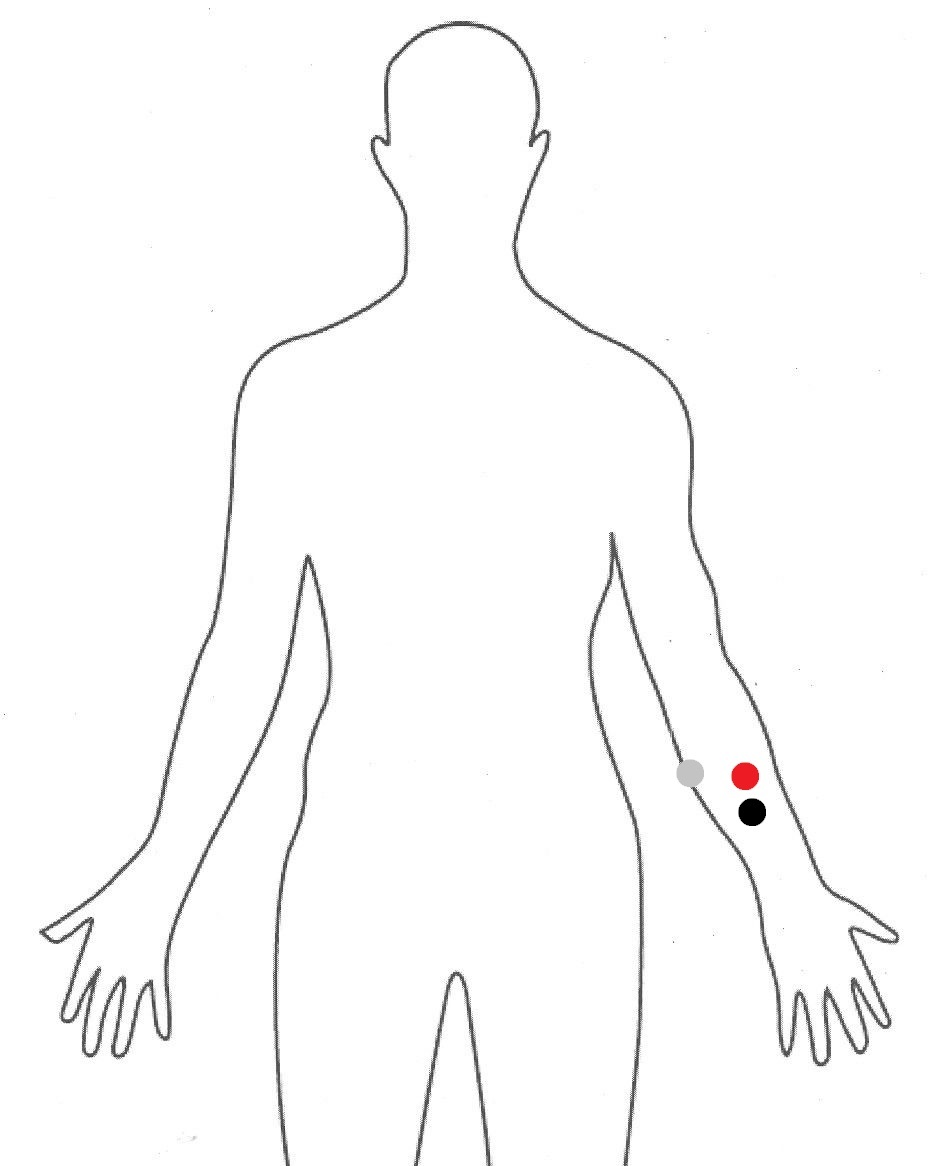
\includegraphics[height=0.3\textheight]{images/bitalino_placement.jpg}
	\caption{Sposób przypięcia elektrod dla sensora EMG,  kolor czerwony oznacza elektrodę dodatnią, czarny ujemną, a~szary elektrodę referencyjną}
	\label{fig:bitalino_placement}
\end{figure}

\section{Dualshock 4}
krótko o~urządzeniu, wykorzystanie akcelerometru do odczytu pobudzenia gracza
